
%(BEGIN_QUESTION)
% Copyright 2015, Tony R. Kuphaldt, released under the Creative Commons Attribution License (v 1.0)
% This means you may do almost anything with this work of mine, so long as you give me proper credit

\noindent
{\bf Lab Exercise} 

\vskip 5pt

Your team's task is to automate a ``process unit'' consisting of tubes, vessels, a measuring transmitter, a final control element, and other components.  At the conclusion of this lab exercise your team's process unit will be controlled by a loop controller so as to maintain its {\it process variable} at some operator-determined {\it setpoint} value.  The process unit is pre-assembled for you -- all your team needs to do is connect it to the controller and properly configure that controller.

During this lab exercise you will not study each system component in detail.  The time will come to study each loop component in depth, in subsequent courses.  For now, you are just learning how the various devices interconnect to form a functional control system.  This will give you perspective and context for your later studies.  A very similar exercise of automating a simple process will be repeated at the end of every quarter (except Summer) by each student individually as a ``capstone'' activity.

The following table of objectives show what you and your team must complete within the scheduled time for this lab exercise.  Note how some of these objectives are individual, while others are for the team as a whole:

\vskip 10pt

\underbar{Objective completion table:}

% No blank lines allowed between lines of an \halign structure!
% I use comments (%) instead, so that TeX doesn't choke.

$$\vbox{\offinterlineskip
\halign{\strut
\vrule \quad\hfil # \ \hfil & 
\vrule \quad\hfil # \ \hfil & 
\vrule \quad\hfil # \ \hfil & 
\vrule \quad\hfil # \ \hfil & 
\vrule \quad\hfil # \ \hfil & 
\vrule \quad\hfil # \ \hfil & 
\vrule \quad\hfil # \ \hfil \vrule \cr
\noalign{\hrule}
%
% First row
{\bf Performance objective} & {\bf Grading} & {\bf 1} & {\bf 2} & {\bf 3} & {\bf 4} & {\bf Team} \cr
%
\noalign{\hrule}
%
% Another row
Manual control of final control element (FCE) & mastery & -- & -- & -- & -- &  \cr
%
\noalign{\hrule}
%
% Another row
Transmitter senses process variable & mastery & -- & -- & -- & -- &  \cr
%
\noalign{\hrule}
%
% Another row
Process is stable in automatic mode & mastery & -- & -- & -- & -- &  \cr
%
\noalign{\hrule}
%
% Another row
Loop calibrator sourcing signal to FCE & mastery & -- & -- & -- & -- &  \cr
%
\noalign{\hrule}
%
% Another row
Loop calibrator reading transmitter signal (live) & mastery & -- & -- & -- & -- &  \cr
%
\noalign{\hrule}
%
% Another row
Loop calibrator simulating transmitter (live) & mastery & -- & -- & -- & -- &  \cr
%
\noalign{\hrule}
%
% Another row
Loop diagram and inspection & mastery &  &  &  &  & -- -- -- -- \cr
%
\noalign{\hrule}
%
% Another row
Connect a tube to a Swagelok style fitting & mastery &  &  &  &  & -- -- -- -- \cr
%
\noalign{\hrule}
%
% Another row
Lab question: Instrument connections & proportional &  &  &  &  & -- -- -- -- \cr
%
\noalign{\hrule}
%
% Another row
Lab question: Commissioning & proportional &  &  &  &  & -- -- -- -- \cr
%
\noalign{\hrule}
%
% Another row
Lab question: Mental math & proportional &  &  &  &  & -- -- -- -- \cr
%
\noalign{\hrule}
%
% Another row
Lab question: Diagnostics & proportional &  &  &  &  & -- -- -- -- \cr
%
\noalign{\hrule}
%
% Another row
Decommission and lab clean-up & mastery & -- & -- & -- & -- &  \cr
%
\noalign{\hrule}
%
% Another row
Personal tool kit complete (show on last day) & mastery &  &  &  &  & -- -- -- -- \cr
%
\noalign{\hrule}
%
% Another row
Reply to email message on BTC account & mastery &  &  &  &  & -- -- -- -- \cr
%
\noalign{\hrule}
} % End of \halign 
}$$ % End of \vbox

The only ``proportional'' scoring in this activity are the lab questions, which are answered by each student individually.  A listing of potential lab questions are shown at the end of this worksheet question.  The lab questions are intended to guide your labwork as much as they are intended to measure your comprehension, and as such the instructor may ask these questions of your team day by day, rather than all at once (on a single day).

\vskip 10pt

{\bf It is essential that your team plans ahead what to accomplish each day.  A short (10 minute) team meeting at the beginning of each lab session is a good way to do this, reviewing what's already been done, what's left to do, and what assessments you should be ready for.  There is a lot of work involved with building, documenting, and troubleshooting these working instrument systems!}

As you and your team work on this system, you will invariably encounter problems.  You should always attempt to solve these problems as a team before requesting instructor assistance.  If you still require instructor assistance, write your team's color on the lab whiteboard with a brief description of what you need help on.  The instructor will meet with each team in order they appear on the whiteboard to address these problems.











\vfil \eject

\noindent
{\bf Lab Exercise -- safety first!}

\vskip 30pt

\noindent
Before you begin working in the lab room, let's identify the locations of some important items:

\begin{itemize}
\item{} First-aid kit (near the north-west exterior door)
\vskip 10pt
\item{} Fire extinguisher (near the main lab entrance door)
\vskip 10pt
\item{} Chemical shower (near the main lab entrance door)
\vskip 10pt
\item{} Sink with eyewash nozzles (on the south end of the lab)
\vskip 10pt
\item{} Emergency power shut-off buttons (near the main lab entrance door)
\vskip 10pt
\item{} Emergency procedures handbook (on the south end of the main control panel)
\vskip 10pt
\item{} Danger tags, for tagging out equipment (near the main control panel)
\vskip 10pt
\item{} Extra safety glasses and goggles (near the instructors' office doors)
\vskip 10pt
\item{} Step-ladders (north-east corner of lab room)
\end{itemize}

\vskip 30pt

\noindent
You must adhere to these safety rules at all times when working in the lab:

\begin{itemize}
\item{} No open-toed shoes (e.g. sandals) allowed in the lab!
\vskip 10pt
\item{} Eye protection must be worn at all times in the lab room!
\vskip 10pt
\item{} Never use a power tool you are unfamiliar with.  Get assistance from the instructor before using it for the first time!  An instructor must be present in the room if you are using a power tool.
\vskip 10pt
\item{} No work with dangerous voltages (anything greater than 30 volts) without an instructor present in the room!
\vskip 10pt
\item{} Hearing protection must be worn when working around or with loud tools!
\item{} Chop saw
\item{} Hand drill (using hole saw)
\vskip 10pt
\item{} Always use a step-ladder, never a chair, to reach for something in a high location!
\end{itemize}

\vskip 20pt

An important safety policy at many industrial facilities is something called {\it stop-work authority}, which means any employee has the right to stop work they question as unsafe.  The same applies in this lab: each and every student has the authority to stop work if they feel in any way unsafe!








\vfil \eject

\noindent
{\bf Lab Exercise -- process unit options}

\vskip 5pt

Several different process units have been constructed for your use, a number of them mounted to 2' $\times$ 2' plywood boards for convenient placement within racks at different points in the lab room.  The following photographs show a couple of process unit examples.

\vskip 10pt

\noindent
{\bf Air pressure control process}

$$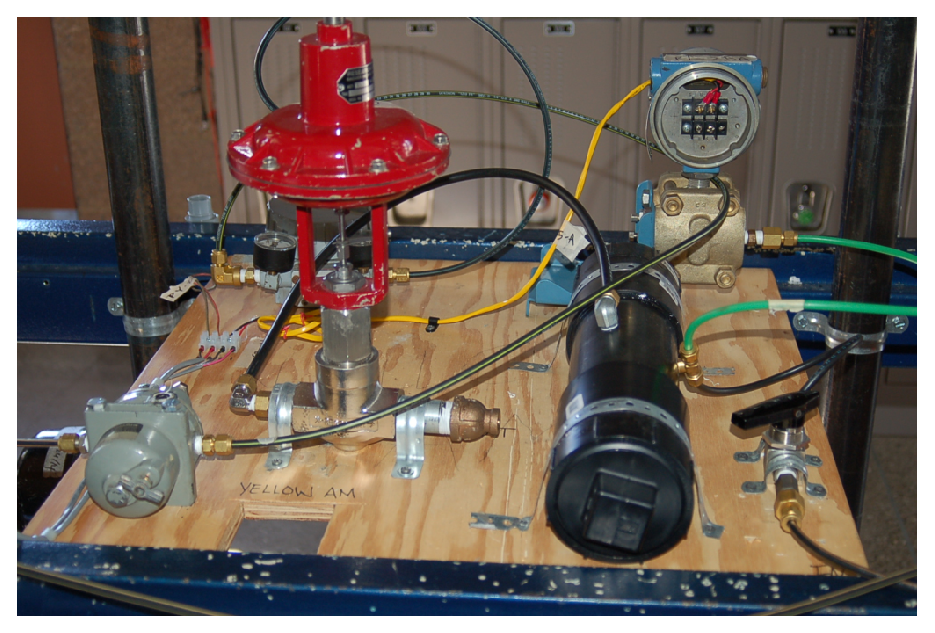
\includegraphics[width=15.5cm]{i00062x01.eps}$$

In this particular process, a hand-operated valve (black handle) introduces compressed air into a vessel (black ABS plastic cylinder) while a pneumatically controlled valve (red) vents air from that vessel to the atmosphere.  A transmitter (blue) senses the amount of accumulated air pressure inside the vessel and reports it to the controller, which in turn sends an electrical signal to a current-pressure converter (grey) modulating air pressure to the red control valve.  By throttling the red control valve, the loop controller is able to maintain a steady air pressure inside the black plastic vessel despite changes in the hand valve's position or changes in the supplied air pressure.

\vskip 10pt

This is an example of a process requiring {\it direct} controller action: if the air pressure inside the vessel \underbar{exceeds} the setpoint value (i.e. there is too much air pressure in the vessel), the controller must \underbar{increase} its signal to the control valve in order to vent more air out of the vessel and thereby decrease the vessel's pressure.  



\vskip 10pt

\filbreak

\noindent
{\bf Turbine speed control process}

$$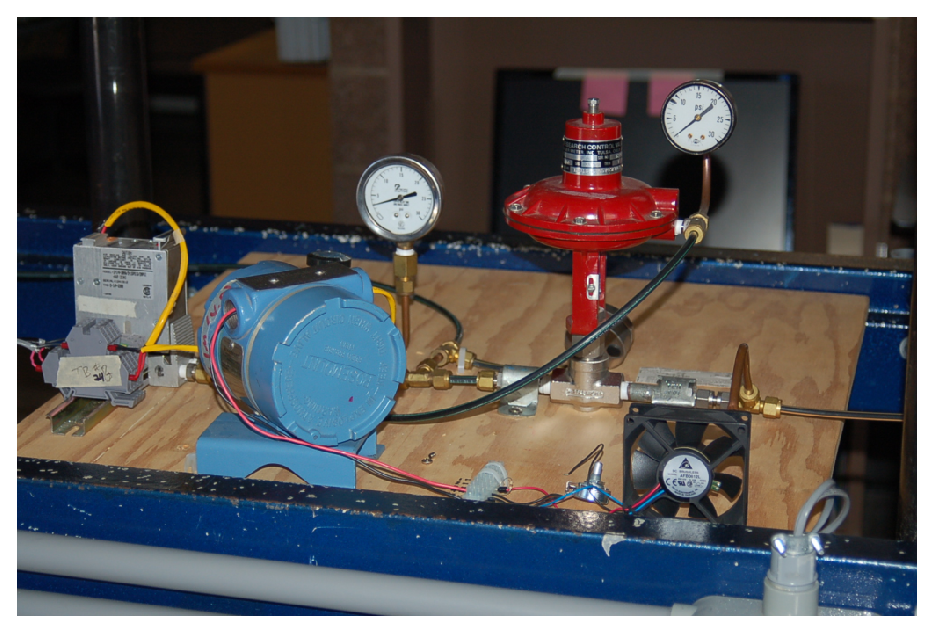
\includegraphics[width=15.5cm]{i00062x02.eps}$$

In this particular process, compressed air exiting a nozzle (bent copper tube) impinges on the blades of a turbine (7-bladed fan), spinning it to create a small amount of DC voltage.  A transmitter (blue) senses that voltage and reports it to the controller, which in turn sends an electrical signal to a current-pressure converter (silver box) modulating air pressure to a pneumatically actuated valve (red) throttling compressed air to the nozzle.  By throttling this red control valve, the loop controller is able to maintain a steady turbine speed despite changes in supplied air pressure or mechanical loading of the turbine.

\vskip 10pt

This is an example of a process requiring {\it reverse} controller action: if the turbine's speed \underbar{exceeds} the setpoint value (i.e. it is spinning too fast), the controller must \underbar{decrease} its signal to the control valve in order to discharge less compressed air out of the nozzle and thereby slow the turbine down.

\vskip 10pt

One of the tasks of an instrument technician is to determine the necessary controller action from an analysis of the process.  For this reason it will be your team's responsibility to determine the needed action and to configure your controller accordingly -- your instructor will not determine this for you.











\vfil \eject

\noindent
{\bf Lab Exercise -- commissioning the system (connecting final control element to loop controller output)}

\vskip 5pt

The Instrumentation lab is equipped to facilitate the construction of working instrument ``loops,'' with over a dozen junction boxes, pre-pulled signal cables, and ``racks'' set up with 2-inch vertical pipes for mounting instruments and 2' by 2' process units.  The only wires you should need to install to build a working system are those connecting the field instrument to the nearest junction box, and then small ``jumper'' cables connecting different pre-installed cables together within intermediate junction boxes.

It is simplest to begin the commissioning of your process unit by first connecting the final control element to the loop controller.  If your team's process unit uses a pneumatically actuated control valve, then the controller's 4-20 mA signal will connect to an ``I/P'' current-to-pressure converter which should already be tubed to the valve's actuating diaphragm.  If your team's process unit uses some other final control element such as an electric heater or a motor speed drive, the controller's 4-20 mA signal will connect to those instead.  In any case, the process unit will be equipped with a terminal block ready to accept the controller's 4-20 mA output signal.

Your process may require compressed air to function.  Clean, dry ``instrument air'' is available at all utility columns in the lab room, and along some of the instrument racks as well (through stainless-steel tubes).  Make the connection between the nearest air supply and the process unit using a length of plastic tubing with pre-attached tube fitting nuts and ferrules at the end.  To see how tube fittings are assembled, you might want to inspect one of the pre-built systems in the lab to see how tubes are attached to instruments there.

\vskip 10pt

You have several options for loop controllers in the lab room: {\it panel-mounted} controllers (located on the main control panel), remote-mounted {\it PLC} units (located in some of the junction boxes), and the lab's {\it DCS} with two ``nodes'' located at the north and south ends of the lab room.  You will need to consult documentation for each of these loop controller types to see which terminals you connect the valve's signal wiring to.  The PLC and DCS controllers have wiring diagrams located in the junction boxes.  The panel-mounted loop controllers are documented in user's manuals.

Once the final control element has been successfully connected to the loop controller's output terminals, you may place the controller in ``Manual'' mode and use it to command the FCE through its full range of action.  This is the first ``loop check'' test of your team's system.

\vskip 10pt

If you experience any trouble along the way, use your multimeter to diagnose the location of the problem.  Bear in mind that the loop controller behaves as an electrical {\it source} while the FCE behaves as an electrical {\it load} to the 4-20 mA signal.










\vfil \eject

\noindent
{\bf Lab Exercise -- commissioning the system (pipe versus tube fittings)}

\vskip 5pt

One of the ``just-in-time'' learning activities students encounter in their first loop construction exercise is how to deal with {\it pipe} versus {\it tube} fittings.  Those students familiar with household plumbing will already be familiar with pipe fittings, but instrument tube fittings are new to almost all new students.

\vskip 10pt

A {\it pipe} fitting is designed to join rigid metal pipes to other metal pipes and/or to instruments with fluid pressure ports.  Standard American pipe threads are {\it tapered}, which means they achieve a leak-free connection by tightening with significant torque.  An essential detail to address with pipe fittings is how to seal and lubricate these tapered threads.  This is done by applying either {\it pipe thread compound} (pipe ``dope''), {\it Teflon tape}, or other sealant materials to the mating threads prior to assembly.  Failure to apply sealant to pipe threads will result in leaks and possibly damaged pipe fittings!

\vskip 10pt

By contrast, a {\it tube} fitting is designed to join rigid or flexible tubes to other tubes and/or to pipe threads.  Instrument-grade tube fittings achieve a seal by using {\it compression} to force a small metal ring (called the {\it ferrule}) to grip the circumference of a tube with just the right amount of tension.  Instrument tube fitting threads are {\it straight} (not tapered), which means they do not become progressively tighter in the same way tapered pipe fittings do.  No thread sealant (e.g. Teflon tape) is required to make tube fittings seal, just the proper amount of compression.  In fact, thread sealant actually gets in the way of making a good seal with instrument tube fittings.  

The standard amount of tightening for initial assembly of 1/4 inch and 3/8 inch Swagelok brand instrument tube fittings (``swaging'' the ferrule around the tube for the first time) is one and one-quarter turns (1-1/4 turns).  Re-making a tube fitting requires only that the nut be ``snugged,'' not re-tightened 1-1/4 turns!

\vskip 10pt

For more detail on this important subject, refer to the ``Pipe and Pipe Fittings'' and ``Tube and Tube Fittings'' sections of the ``Instrument Connections'' chapter of your {\it Lessons In Industrial Instrumentation} textbook.  Other good resources include documentation from pipe and tube fitting manufacturers.  Both Swagelok and Parker publish free guides on the assembly and use of both types of fittings.










\vfil \eject

\noindent
{\bf Lab Exercise -- commissioning the system (connecting transmitter to loop controller input)}

\vskip 5pt

The next step in building your team's loop is to connect the process unit's sensing device (the ``transmitter'') to the loop controller.  A suitable transmitter will already be mounted on the process unit, ready to connect.  As with the final control element, the process unit will be equipped with a terminal block ready to accept wires connecting the transmitter to the controller's 4-20 mA input terminals.

As with the valve's control wiring, the only wires you should need to install to connect the transmitter to the controller are those connecting the field instrument to the nearest junction box, and then small ``jumper'' cables connecting different pre-installed cables together within intermediate junction boxes.  The pre-installed multi-conductor cables will span most of the distance between your transmitter and your loop controller.

Consult manufacturer's documentation to see how to make the wiring connections between the transmitter and the loop controller (consulting the pre-printed wiring diagrams for wiring details on the PLC and DCS controllers).  You may find user's manuals for the pressure transmitters online (the Internet).

\vskip 10pt

Once the transmitter has been successfully connected to the loop controller's output terminals, you may actuate the process unit's final control element and monitor the controller's ``process variable'' display to see the indication change.  This is the second ``loop check'' test of your team's system.

\vskip 10pt

If you experience any trouble along the way, use your multimeter to diagnose the location of the problem.  Bear in mind that the loop controller behaves as an electrical {\it source} while the transmitter behaves as an electrical {\it load} to the 4-20 mA signal, even though the transmitter is the component responsible for regulating the amount of current in this circuit.  Such ``loop-powered'' transmitters are typical in process instrumentation.

\vskip 10pt

Note that determining how to connect your process transmitter to the controller input is typically the most confusing aspect of the ``capstone'' assessment (done at the end of Fall, Winter, and Spring quarters).  The reason for this confusion is the diversity of transmitter types (loop-powered versus self-powered) and controller inputs (powered versus unpowered, voltage versus current).  The key to properly determining the correct connections lies in analyzing the transmitter loop as a DC circuit, knowing it must have a DC power source somewhere in it, and identifying each component's function as either a {\it source} or a {\it load} in order to correctly route the 4-20 mA current signal through them all in series fashion.








\vfil \eject

\noindent
{\bf Lab Exercise -- commissioning the system (test in automatic mode)}

\vskip 5pt

After verifying the final control element's operation and the transmitter's ability to sense the process variable, you are ready for the next step: configuring the loop controller to automatically control the process.  

First, you will need to determine the necessary action for the controller: either {\it direct} or {\it reverse}.  This is solely determined by the design of your process unit.  From the previous two tests (FCE test and transmitter test), you should have all the information necessary to determine the effect of the FCE on the process variable.  If the FCE has a direct effect on the PV (i.e. increased output from the controller results in increased PV) then the controller must be configured for reverse action.  If the FCE has a reverse effect on the PV (i.e. increased output results in decreased PV) then the controller must be configured for direct action.

Every loop controller is capable of implementing both types of action.  To change the controller's action, consult the manual for that controller.  It will guide you to finding the proper parameter defining controller action.

Once the controller's action has been properly configured, you should configure its ``PID tuning'' parameters.  PID tuning is a complex subject, far beyond the scope of this exercise, so for now you will set these parameters to modest values and let your instructor ``tune'' the controller for precise operation.  Consult the manual to find the PID tuning parameters for your team's controller, and then set those parameters as follows:

\begin{itemize}
\item{} {\bf (P)} -- set to a gain of 0.5, or a ``proportional band'' of 200\%
\item{} {\bf (I)} -- set to minimum effect (very small repeats per minute, or very large minutes per repeat)
\item{} {\bf (D)} -- set to minimum effect (zero minutes)
\end{itemize}

After the loop controller's action and PID tuning parameters have been properly configured, you are ready to try operating the process in automatic mode.  Begin by placing the controller in ``Manual'' mode and moving the output to such a point that the process variable reads approximately 50\% of scale.  Once that point has been reached, switch the controller from ``Manual'' mode to ``Automatic'' mode.  If all is well, the process variable should remain fairly constant, the controller making automatic corrections to its output signal to maintain the PV at or near setpoint.

Successful demonstration of automatic-mode operation is the third ``loop check'' of your team's system.

\vskip 10pt

{\bf If a team is working efficiently, they should be able to commission a process unit within the span of one 3-hour lab session.}








\vfil \eject

\noindent
{\bf Lab Exercise -- using a loop calibrator}

\vskip 5pt

Aside from your multimeter, one of the most important tools for the instrument technician to master is the {\it loop calibrator}.  These are special milliammeters equipped with the ability to {\it generate} 4-20 milliamp signals as well as measure them.  As a team, you and your teammates will demonstrate the use of a loop calibrator to do the following tasks while correctly identifying electrical properties such as {\it source} versus {\it load}, voltage polarities, and current directions (conventional flow) with the loop calibrator connected to the circuit:

\vskip 10pt

\begin{itemize}
\item{} {\it Measure} the 4-20 mA signal sent by the transmitter to the controller, identifying all electrical \underbar{sources} and \underbar{loads} and also properly identifying \underbar{voltage polarities} and \underbar{current} directions in the circuit
\vskip 15pt 
\item{} {\it Source} a 4-20 mA signal to the final control element (taking the place of the controller), identifying all electrical \underbar{sources} and \underbar{loads} and also properly identifying \underbar{voltage polarities} and \underbar{current directions} in the circuit
\vskip 15pt 
\item{} {\it Simulate} a transmitter to send your own 4-20 mA signal to the controller, identifying all electrical \underbar{sources} and \underbar{loads} and also properly identifying \underbar{voltage polarities} and \underbar{current directions} in the circuit
\end{itemize}

\vskip 10pt

Details on the use of loop calibrators and their electrical functions may be found in the ``Using Loop Calibrators'' subsection of the ``Troubleshooting Current Loops'' section of the ``Analog Electronic Instrumentation'' chapter in your {\it Lessons In Industrial Instrumentation} textbook.

\vskip 10pt

In this lab exercise, your team will be asked to demonstrate the use of a loop calibrator on the connected process unit, and to do so in a way that is realistic to the profession.  This means using the calibrator in such a way as to avoid any detrimental effect on the process.

When {\it sourcing} a 4-20 mA signal to the final control element, you should first secure all energy sources that would make the process respond to that 4-20 mA signal in order to ensure the process variable cannot reach unsafe levels.  For example, if your process happens to be a turbine speed control, you should shut off any manual valves that would allow air to reach the nozzle and potentially make the turbine spin out of control when the control valve is actuated by the loop calibrator's signal.  

When {\it measuring} the 4-20 mA signal sent by the transmitter, you should do so while the process is running in order to emulate a real-world condition where you as an instrument technician must diagnose problems on ``live'' processes.  Of course, disconnecting any portion of the 4-20 mA transmitter circuit will interrupt the PV signal sent to the controller, which may be disastrous for a running process with the controller in automatic mode.  Therefore, you will need to place the controller in manual mode before performing this test, and return the controller to automatic mode after reconnecting the wires at the conclusion of the test.  A loop controller placed in manual mode ignores the PV signal and maintains the output at whatever value the human operator desires, which is what allows you to interrupt that PV signal and perform your signal measurement without adversely affecting the process.

When {\it simulating} the transmitter with a loop calibrator, you should similarly place the controller in manual mode before performing the test.  This will prevent the controller from taking action on false information (as you simulate the transmitter responding over its full range of measurement) and potentially driving the real process variable to unsafe levels.  Return the controller to automatic mode at the conclusion of your test.

If your process unit happens to be equipped with manual ``block'' and ``bypass'' valves around the control valve, it it possible to perform the {\it current sourcing} test on the control valve with the process running.  The procedure for doing so is as follows: (1) Slowly open the bypass valve with the controller in automatic mode and let the controller shut off the control valve as it holds PV = SP.  (2) Once the control valve has reached the fully shut position, switch the controller to manual mode and close both block valves.  (3) Disconnect the FCE wires from the controller and connect to the loop calibrator.  (4) Perform the test using the loop calibrator to ``stroke'' the control valve throughout its range.  (5) Reconnect the FCE wires to the controller's output and verify control valve operation by stroking the valve through its whole range using the controller's adjustable output in manual mode.  (6) Return the valve to its fully-closed position in manual mode and open the block valves.  (7) Switch the controller to automatic mode.  (8) Slowly close the bypass valve and let the controller open up the control valve as it holds PV = SP.

\vskip 10pt

Loop calibrators, along with some other specialized tools, may be found in the {\it team tool locker}.  Each team has a color-designated locker in the lab room containing certain specialized tools you are not expected to own.  Each team is responsible for ensuring these tools get put back into the locker at the end of each lab session, that the locker is locked at the end of each lab session, that all tools are kept in good working order, and also that the tool lockers remain free of personal items.  Each tool locker will be inspected at the end of the quarter, with team members held responsible for replacing any missing tools at their own expense.

It should be noted that each locker contains an itemized list of all contents, which should be periodically checked to ensure nothing is missing.









\vfil \eject

\noindent
{\bf Lab Exercise -- documenting the system}

\vskip 5pt

Each student must sketch their own {\it loop diagram} for their team's system, following proper ISA conventions.  Sample loop diagrams are shown in the next question in this worksheet, and a loop diagram ``template'' is included at the end of this question (although this template may not precisely match the instruments you have chosen for your loop).  These loop diagrams must be {\it comprehensive} and {\it detailed}, showing every wire connection, every cable, every terminal block, range points, etc.  The principle to keep in mind here is to make the loop diagram so complete and unambiguous that anyone can follow it to see what connects to what, even someone unfamiliar with industrial instrumentation.  In industry, loops are often constructed by contract personnel with limited understanding of how the system is supposed to function.  The loop diagrams they follow must be so complete that they will be able to connect everything properly without necessarily understanding how it is supposed to work.

Every instrument and every signal cable in your loop needs to be properly labeled with an ISA-standard tag number.  An easy way to do this is to wrap a short piece of masking tape around each cable (and placed on each instrument) then writing on that masking tape with a permanent marker.  Although no industry standard exists for labeling signal cables, a good recommendation is to label each two-wire cable with the tag number of the field instrument it goes to.  Thus, every length of two-wire cable in a pressure transmitter circuit should be labeled ``PT-$x$'' (where ``$x$'' is the loop number), every flow control valve should be labeled ``FV-$x$'', etc.  Remember that the entire loop is defined by the process variable it measures: if the PV is {\it temperature} then the transmitter with be a {\it T}T, the control valve will be a {\it T}V, the controller with be a {\it T}C, etc.

When your entire team is finished drafting your individual loop diagrams, call the instructor to do an inspection of the loop.  Here, the instructor will have students take turns going through the entire loop, with the other students checking their diagrams for errors and omissions along the way.  During this time the instructor will also inspect the quality of the installation, identifying problems such as frayed wires, improperly crimped terminals, poor cable routing, missing labels, lack of wire duct covers, etc.  The team must correct all identified errors in order to receive credit for their system.  

After successfully passing the inspection, each team member needs to place their loop diagram in the diagram holder located in the middle of the lab behind the main control panel.  When it comes time to troubleshoot another team's system, this is where you will go to find a loop diagram for that system!

\vskip 10pt

{\bf Common mistakes:}

\begin{itemize}
\item{} Forgetting to label all signal wires (see example loop diagrams).
\item{} Forgetting to label all field instruments with their own tag names (e.g. PT-83, PIC-83, PV-83).
\item{} Forgetting to note all wire colors.
\item{} Forgetting to put your name on the loop diagram!
\item{} Basing your diagram off of a team-mate's diagram, rather than closely inspecting the system for yourself.
\item{} Not placing loop sheet instruments in the correct orientation (field instruments on the left, control room instruments on the right).
\end{itemize}

\vskip 10pt

{\bf Creating and inspecting accurate loop diagrams should take no more than one full lab session (3 hours) if the team is working efficiently!}









\vfil \eject

\noindent
{\bf Lab questions}

\vskip 5pt

It is each team's responsibility to study for these lab questions, and to be prepared to answer them throughout the loop construction and testing process.  These questions serve not only to measure your progress, but also to {\it guide} your progress as you construct, test, and diagnose your loop systems.  Teams are encouraged to review this question list during each lab session's initial planning time, to assess how far they have progressed in their understanding of the system and how far they still need to go.

Certain lab questions such as those under ``Instrument installation'' should be answerable by every team member as soon as the loop is constructed.  The instructor will meet with each team to quiz them on these lab questions at appropriate times throughout the multi-day lab exercise.  Doing this helps encourage each team to progress at a good pace, stay abreast of the learning objectives, and also avoid a ``rush'' at the final deadline date for answering all lab questions.

\vskip 10pt

\begin{itemize}
\item{} {\bf Instrument connections}
\item{} Determine correct wire connections between instruments to create a working 4-20 mA loop circuit, based on diagrams of instruments with terminals labeled
\item{} Correctly determine all electrical sources and loads, as well as all voltage polarities and current directions in a 4-20 mA loop circuit, based on diagrams of instruments with terminals labeled
\end{itemize}

\filbreak

\begin{itemize}
\item{} {\bf Commissioning and Documentation}
\item{} Demonstrate how to isolate potentially hazardous energy in your system ({\it lock-out, tag-out}) and also how to safely verify the energy has been isolated prior to commencing work on the system
\item{} Demonstrate how a sound electrical connection is made at each terminal block
\item{} Identify the ``high'' and ``low'' pressure ports on a pressure transmitter, and explain their significance
\item{} Explain the difference between {\it direct} and {\it reverse} controller action
\item{} Explain in simple terms how a varying air pressure actuates the control valve mechanism
\item{} Identify multiple locations (referencing a loop diagram) you may measure various 4-20 mA instrument signals in the system
\end{itemize}

\filbreak


\begin{itemize}
\item{} {\bf Mental math} (no calculator allowed!)
\item{} Calculate the pneumatic pressure in a 3-15 PSI range corresponding to $x$ percent.
\item{} Calculate the electrical current in a 4-20 mA range corresponding to $x$ percent.
\item{} Calculate the electrical voltage in a 1-5 volt range corresponding to $x$ percent.
\item{} Calculate the percentage value of a pneumatic pressure signal $x$ PSI in a 3-15 PSI range.
\item{} Calculate the percentage value of an electrical current signal $x$ mA in a 4-20 mA range.
\item{} Calculate the percentage value of an electrical voltage signal $x$ volts in a 1-5 volt range.
\end{itemize}

\filbreak


\begin{itemize}
\item{} {\bf Diagnostics}
\item{} Given a particular component or wiring fault ({\it instructor specifies type and location}), what symptoms would the loop exhibit and why?
\item{} Determine whether or not a given diagnostic test will provide useful information, given a set of symptoms exhibited by a failed system
\item{} Identify at least two plausible faults given the results of a diagnostic test and a set of symptoms exhibited by a failed system
\item{} Propose a diagnostic test for troubleshooting a failed system and then explain the meanings of two different test results
\end{itemize}

% FUTURE ADDITION: lesson on the proper uses of Teflon pipe tape, and the differences between tube, pipe, and conduit threads.













\vfil \eject

\noindent
{\bf Lab Exercise -- decommissioning and clean-up}

\vskip 5pt

The final step of this lab exercise is to decommission your team's entire system and re-stock certain components back to their proper storage locations, the purpose of which being to return the lab facility to the state in which you found it (or better!) when you began this lab exercise.  This includes, but is not limited to:

\begin{itemize}
\item{} Returning the process unit to its proper storage location
\item{} Returning all wires and tubes to their storage locations
\item{} Resetting all controller parameters to their default values
\item{} Returning tools to the team tool locker
\item{} Removing your loop diagrams from the common holding area
\item{} Removing all temporary labels from instruments, cables, etc.
\item{} General clean-up (removal of all trash, sweeping floors, etc.)
\end{itemize}

{\bf Note: the process unit should be returned to its storage location in fully operational condition, so it will be ready for immediate use in the next lab exercise!}












\vfil \eject

\noindent
{\bf Lab Exercise -- tool kit and email usage}

\vskip 5pt

Two additional objectives that are not technically a part of making this lab project function, but are nevertheless very important to your continued success in the Instrumentation program, include assembling a personal tool kit and using your BTC email account (which is automatically created for every student at the college).  

\vskip 10pt

You will be using your tool kit throughout the remainder of this program, and so it is very important to have it complete and ready to use by the end of this lab exercise.  Note that there are several optional items listed in addition to mandatory items.  These optional tools are useful, but not 100\% necessary for the work you will be doing in the lab.  Also note that there are some consumable items in your tool list such as electrical compression terminals which you will need to keep stocked as you use them in your labwork.

\vskip 10pt

Likewise, you will be relying on email to receive important messages from your instructor(s) throughout the remainder of the program.  These messages include, but are not limited to, job announcements, guest speaker appearances, schedule changes, emergency notifications, scholarship announcements, and feedback on your personal performance in the program.  The reason we use email as opposed to using learning management software is because it is imperative you learn how to appropriately use email for your chosen career.  Email is simply the most common and most practical medium businesses use for day-to-day electronic communication.  

Every BTC student is automatically given an email account upon registration, and this account remains active for some time after graduation.  If you would rather not add one more email account to your electronic life, there is the option of having all messages received in your BTC email inbox automatically forwarded to the email platform of your choice (Yahoo, Hotmail, Gmail, Live, etc.) which may be selected as an option within your BTC email management webpage.  {\it It is your responsibility to log in to your BTC email account, set up any forwarding features you would like, and to check your email account daily to receive these important messages.}

The library staff at BTC provide technical support for all school-related IT (Information Technology) needs.  If you are experiencing trouble with your email account, with password management, or any other network-based technology necessary for your learning at BTC, the library staff are well-trained and helpful in this regard.

{\bf Your readiness for email use will be assessed by your reply to an email message sent to you by your instructor.  Replying to this email message with an email message of your own is a mastery-level objective for every new student in this lab exercise.}

When you graduate from this program and enter the workforce, your BTC email account will remain active for some time, but not in perpetuity.  Therefore, you must inform your instructors of your preferred email account for post-graduation correspondence before you leave BTC.  We use email to regularly communicate job announcements of interest to graduates, so it is in your best interest to remain connected.

\vskip 10pt



\underbar{file i00062}
%(END_QUESTION)





%(BEGIN_ANSWER)



%(END_ANSWER)





%(BEGIN_NOTES)

\vfil \eject

\noindent
{\bf Lab questions}

\vskip 20pt

\item{$(1)$} Sketch wire connections necessary for this pressure transmitter to send a process variable signal to the Foxboro controller.  Note that the transmitter is {\it loop-powered} (2-wire, 4-20 mA):

$$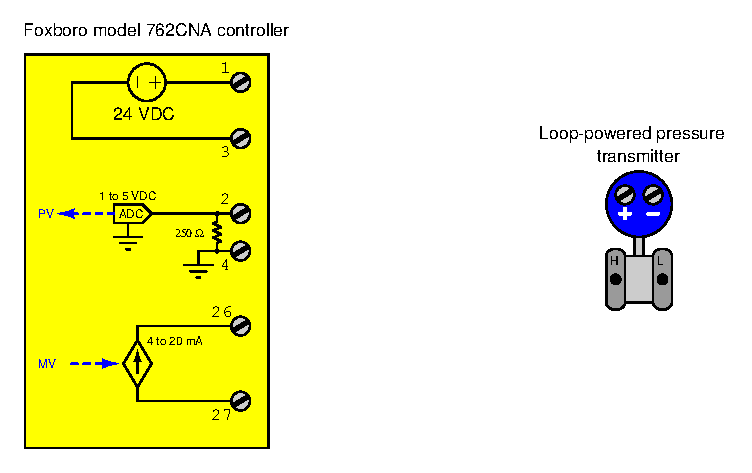
\includegraphics[width=15.5cm]{i00062x03.eps}$$

\vskip 20pt

\item{$(2)$} Describe how to visually identify the ``high'' and ``low'' pressure ports on a pressure transmitter, and explain their significance.

\vskip 20pt

\item{$(3)$} Calculate the percentage value represented by a 7 PSI pneumatic pressure signal in a 3-15 PSI range.

\vskip 20pt

\item{$(4)$} A 4-20 mA loop-powered pressure transmitter connects to a 4-20 mA electronic indicator.  Both instruments are supposed to be ranged for 0 to 300 PSI.  When the transmitter senses an actual process pressure of 110 PSI, however, the indicator registers 125 PSI instead.  An instrument technician measures current in this 4-20 mA circuit during these conditions (i.e. process pressure = 110 PSI and indication = 125 PSI) and obtains a reading of 9.87 milliamps.  Identify where the problem is most likely located in this pressure measurement system.






\vfil \eject

\noindent
{\bf Lab questions}

\vskip 20pt

\item{$(1)$} Sketch wire connections necessary for this liquid level transmitter to send a process variable signal to the Foxboro controller.  Note that the transmitter is {\it self-powered} (4-wire, 4-20 mA):

$$\includegraphics[width=15.5cm]{i00062x04.eps}$$

\vskip 20pt

\item{$(2)$} Explain the difference between {\it direct} and {\it reverse} controller action, using an example if you find it helpful.

\vskip 20pt

\item{$(3)$} Calculate the percentage value represented by a 13 mA analog electronic signal in a 4-20 mA range.

\vskip 20pt

\item{$(4)$} A level-indicating controller (LIC) receives its process variable signal from a loop-powered 4-20 mA electronic level transmitter configured for a range of 0 to 200 inches.  The system was working fine for years, but then one day the LIC began to register $-50$ inches all the time regardless of the actual process liquid level.  Measuring voltage across the transmitter terminals, you see your meter indicate 0 volts DC.  Two technicians working with you offer different analyses: one of them tells you the cable between the transmitter and the controller must be failed open, while the other insists the cable must be failed shorted.  What do you think might account for all the symptoms in this system?  Explain your answer in detail.




%INDEX% Lab exercise, introduction to feedback control loops

%(END_NOTES)


